\documentclass[11pt,a4paper]{article}
\usepackage[margin=2.3cm]{geometry}
\usepackage[T1]{fontenc}
\usepackage{lmodern}
\usepackage{amsmath,amssymb,bm}
\usepackage{url}
\usepackage{graphicx}
\usepackage{booktabs}
\usepackage[hidelinks]{hyperref}
\usepackage[font=small,labelfont=bf]{caption}

\newcommand{\tr}{\operatorname{Tr}}
\newcommand{\Lc}{\mathcal{L}}

\title{Exact deepest-tier elimination for stationary HEOM:\\
a converged low-temperature benchmark for a correlated Anderson-impurity quench}
\author{Hugo Wei\\[2pt]
\small CentraleSupélec \& ESCP Business School, Paris\\
\small \texttt{github.com/HugoWEI/nonmarkovian-neural-dynamics}}
\date{November 2026}

\begin{document}
\maketitle

\begin{abstract}
Hierarchical equations of motion (HEOM) give numerically exact dynamics for an
open quantum system coupled to a Gaussian bath, but the hierarchy grows
combinatorially with depth and with the number of bath exponents. For
quench protocols that start from the \emph{correlated} system--bath stationary
state, preparing that state is often the bottleneck. We note that the deepest
tier of a truncated HEOM is coupled to nothing below it, so its generator block
is block diagonal (exactly diagonal for an impurity Hamiltonian diagonal in the
occupation basis) and can be eliminated by a Schur complement without
approximation. Applied to a spinful interacting Anderson impurity with
Lorentzian leads, this reproduces a direct QuTiP solve to $\le 3\times10^{-13}$
while being up to $163\times$ faster, and it makes hierarchies feasible that
the direct solve cannot handle in 7\,GB of memory. With it we obtain a
benchmark at $T/\Gamma = 0.3$ converged in hierarchy depth and Padé order,
$\langle n_\uparrow\rangle(6\,\mathrm{ps}) = 0.50362 \pm 1\times10^{-5}$, and
show that three Padé poles, as used in earlier low-temperature runs of this project, leave an error of
$1.6\times10^{-3}$. The elimination itself is standard linear algebra; the
contribution is its verified use to produce a reference against which
approximate (e.g.\ neural) solvers can be tested.
\end{abstract}

\section{Motivation}

Non-Markovian open quantum systems---a quantum dot coupled to metallic leads,
a molecule in a solvent, a qubit near a structured environment---have dynamics
that depend on their whole history. HEOM~\cite{TanimuraKubo1989,Tanimura2020}
and its fermionic generalisation~\cite{Jin2008} handle this memory exactly by
encoding the bath's influence in a hierarchy of auxiliary density operators
(ADOs). The price is cost: the number of ADOs grows combinatorially with the
truncation depth and with the number of exponentials used to represent the
bath correlation function, which itself grows as temperature decreases.

Recent work trains neural networks to solve such equations more cheaply. Any
claim that a neural solver is accurate needs a reference that is converged
\emph{independently} of the solver being tested. This note produces one for a
standard test case: an interacting Anderson impurity whose lead chemical
potential is suddenly shifted, starting from the fully correlated stationary
state. At low temperature this reference was out of reach on modest hardware,
because preparing the correlated initial hierarchy required a sparse direct
solve of a system with up to $6.6\times10^{5}$ unknowns.

\section{Model and hierarchy}

\paragraph{System.} A spinful single-level impurity,
\begin{equation}
H_S = \sum_{\sigma}\varepsilon\, n_\sigma + U n_\uparrow n_\downarrow,
\qquad \varepsilon = -0.5\ \mathrm{meV},\quad U = 1\ \mathrm{meV},
\end{equation}
so $\varepsilon = -U/2$ (particle--hole symmetric at $\mu = 0$). Each spin couples to one
fermionic lead with a Lorentzian spectral density of width
$\Gamma = 0.1$\,meV and bandwidth $W = 5$\,meV. The system Hilbert space has
dimension $d = 4$, so each ADO is a $4\times4$ matrix.

\paragraph{Bath expansion.} The lead correlation functions are expanded in
exponentials,
\begin{equation}
C^{\pm}_\sigma(t) = \sum_k \eta^{\pm}_k e^{-\gamma^{\pm}_k t},
\end{equation}
with one Lorentzian pole and $N_k$ Padé poles of the Fermi function~\cite{HuXuYan2010}.
Lower temperature needs more poles, because the Fermi function becomes sharper.
The coefficients were rebuilt from the physical parameters and matched against
published values to numerical precision.

\paragraph{Hierarchy.} Each ADO $\rho_{\mathbf{j}}$ is labelled by a set of
occupied bath exponents; its \emph{tier} is $|\mathbf{j}|$. Truncating at depth
$n$ keeps tiers $0,\dots,n$; tier 0 is the physical reduced density matrix. The
fermionic HEOM has the structure
\begin{equation}
\dot\rho_{\mathbf{j}} = -\Big(i\Lc_S + \sum_{k\in\mathbf{j}}\gamma_k\Big)\rho_{\mathbf{j}}
\;+\;\sum_{k\notin\mathbf{j}}\mathcal{A}_k\,\rho_{\mathbf{j}+k}
\;+\;\sum_{k\in\mathbf{j}}\mathcal{C}_k\,\rho_{\mathbf{j}-k},
\label{eq:heom}
\end{equation}
where $\mathcal{A}_k,\mathcal{C}_k$ are (anti)commutator superoperators with the
impurity creation/annihilation operators. Writing all ADOs as one vector $y$,
$\dot y = \Lc y$. All generators here are built with QuTiP's HEOM
module~\cite{Lambert2023}.

\paragraph{Protocol.} At $\mu = 0$ the correlated stationary hierarchy $y_0$
solves $\Lc(\mu{=}0)\,y_0 = 0$ with $\tr\rho = 1$. The lead chemical potential is
then quenched to $\mu = 0.05$\,meV and $\langle n_\uparrow\rangle(t)$ is
propagated for 6\,ps with an explicit DOP853 integrator ($\mathrm{rtol}=10^{-10}$,
$\mathrm{atol}=10^{-12}$). Using $y_0$ rather than a product state $\rho_S\otimes\rho_B$
matters: system--bath correlations are present before the quench, and copying
only the impurity occupations does not reproduce them.

\section{Exact elimination of the deepest tier}

Order the depth-$(n{+}1)$ vector as $y = (x, u)$, with $x$ the tiers $0,\dots,n$ and
$u$ the deepest tier $n{+}1$. Then
\begin{equation}
\Lc = \begin{pmatrix} A & B\\ C & D\end{pmatrix}.
\end{equation}
By Eq.~\eqref{eq:heom}, an ADO in the deepest tier is coupled \emph{upward} to tier $n$ (block $C$),
but there is no tier $n{+}2$ below it, and ADOs within one tier are not coupled
to each other. Hence $D$ only contains each ADO's own term
$-(i\Lc_S + \sum_{k}\gamma_k)$: it is block diagonal with $d^2\times d^2$ blocks.
For this impurity $H_S$ is diagonal in the occupation basis, so $i\Lc_S$ is
diagonal in the corresponding Liouville basis and $D$ is \emph{exactly diagonal}
(verified numerically: 79{,}360 nonzeros on a 79{,}360-dimensional block, none
off-diagonal). Its entries $-(i(E_a-E_b) + \sum_k\gamma_k)$ have strictly
negative real part, so $D$ is invertible.

At stationarity,
\begin{equation}
A x + B u = 0,\qquad C x + D u = 0
\;\Longrightarrow\; u = -D^{-1}C x,\qquad (A - BD^{-1}C)\,x = 0,\quad \tr\rho = 1.
\label{eq:schur}
\end{equation}
The Schur complement $S = A - BD^{-1}C$ has the size of the depth-$n$ hierarchy
but describes the depth-$(n{+}1)$ stationary state \emph{exactly}: nothing is
truncated or approximated. The deepest tier is then recovered by a diagonal
division. The normalisation is imposed by replacing one row of $S$ with the trace
functional, and the resulting sparse system is solved directly.

This is Gaussian elimination, and it is closely related to the HEOM
\emph{terminators} that close the hierarchy by expressing the last tier through
the one above~\cite{TanimuraWolynes1991,IshizakiTanimura2005}; we claim no new
theory. Two points are worth stressing. (i) For the stationary state the
elimination is exact, not an approximate closure, because $\dot u = 0$ removes
the only term that a terminator has to model. (ii) It does \emph{not} apply to the
dynamics: after the quench, $\dot u\neq 0$ and the deepest tier carries memory,
so time propagation uses the full hierarchy.

\section{Results}

\subsection{Exactness and cost of the stationary state}

Table~\ref{tab:cost} compares the eliminated solve with QuTiP's
\texttt{HEOMSolver.steady\_state()} on the full hierarchy. Where both run, they
agree to between $10^{-15}$ and $3\times10^{-13}$ over \emph{all} ADOs, i.e.\
to linear-algebra precision. The speed-up grows with the problem size, reaching
$163\times$ at $N_k = 7$, depth 3. At depth 4 with $N_k = 5$ the direct solve runs
out of memory on the 7\,GB test machine, while the eliminated solve needs about
1\,GB; the $N_k = 7$, depth 4 hierarchy (41{,}449 ADOs) is solved in 164\,s. For these
the full-hierarchy residual $\|\Lc y_0\|$ is below $10^{-14}$.

\begin{table}[h]
\centering\small
\begin{tabular}{rrrrrrrc}
\toprule
$T/\Gamma$ & $N_k$ & depth & ADOs & unknowns & direct & eliminated & max diff / residual\\
\midrule
3.0 & 3 & 3 & 697 & 11{,}152 & 0.16 s & 0.025 s & $9.1\times10^{-16}$\\
0.3 & 3 & 3 & 697 & 11{,}152 & 0.18 s & 0.030 s & $2.2\times10^{-14}$\\
0.3 & 3 & 4 & 2{,}517 & 40{,}272 & 5.8 s & 0.40 s & $4.7\times10^{-14}$\\
0.3 & 7 & 3 & 5{,}489 & 87{,}824 & 75.1 s & 0.46 s & $3.4\times10^{-13}$\\
0.3 & 5 & 4 & 12{,}951 & 207{,}216 & out of memory & 11.3 s & $\|\Lc y_0\| = 1.2\times10^{-15}$\\
0.3 & 7 & 4 & 41{,}449 & 663{,}184 & --- & 164 s & $\|\Lc y_0\| = 7.3\times10^{-15}$\\
\bottomrule
\end{tabular}
\caption{Correlated stationary state at $\mu=0$: direct QuTiP solve versus
deepest-tier elimination (2 CPU cores, 7\,GB RAM). The last column is the maximum
absolute difference over all ADOs where the direct solve exists, otherwise the
residual of the full-hierarchy generator.}
\label{tab:cost}
\end{table}

\subsection{Convergence of the quench}

Each run starts from its own correlated stationary hierarchy, so the depth
comparison is consistent: initial state and dynamics are truncated at the same
depth. Table~\ref{tab:depth} gives the maximum change of
$\langle n_\uparrow\rangle(t)$ over the 6\,ps window between successive depths.

\begin{table}[h]
\centering\small
\begin{tabular}{rrccc}
\toprule
$T/\Gamma$ & $N_k$ & $2\to3$ & $3\to4$ & $4\to5$\\
\midrule
3.0 & 3 & $6.04\times10^{-5}$ & $1.80\times10^{-6}$ & $1.04\times10^{-8}$\\
0.3 & 3 & $1.66\times10^{-3}$ & $1.75\times10^{-4}$ & $2.37\times10^{-6}$\\
0.3 & 5 & $1.59\times10^{-3}$ & $1.62\times10^{-4}$ & ---\\
0.3 & 7 & $1.59\times10^{-3}$ & $1.61\times10^{-4}$ & ---\\
\bottomrule
\end{tabular}
\caption{Depth convergence: $\max_t|\Delta\langle n_\uparrow\rangle|$ between successive hierarchy depths.}
\label{tab:depth}
\end{table}

Convergence in depth is geometric: at low temperature each extra tier reduces
the change by about $10\times$ and then $70\times$. Low temperature is harder
than high temperature by more than an order of magnitude at every depth, as
expected from the slower Padé modes. The depth error is almost independent of
$N_k$ (at each step, rows 2--4 agree to within 10\%), which justifies using the $N_k = 3$
depth-5 step ($2.4\times10^{-6}$) as the estimate of the remaining depth error at
$N_k = 7$, depth 4.

\begin{figure}[t]
\centering
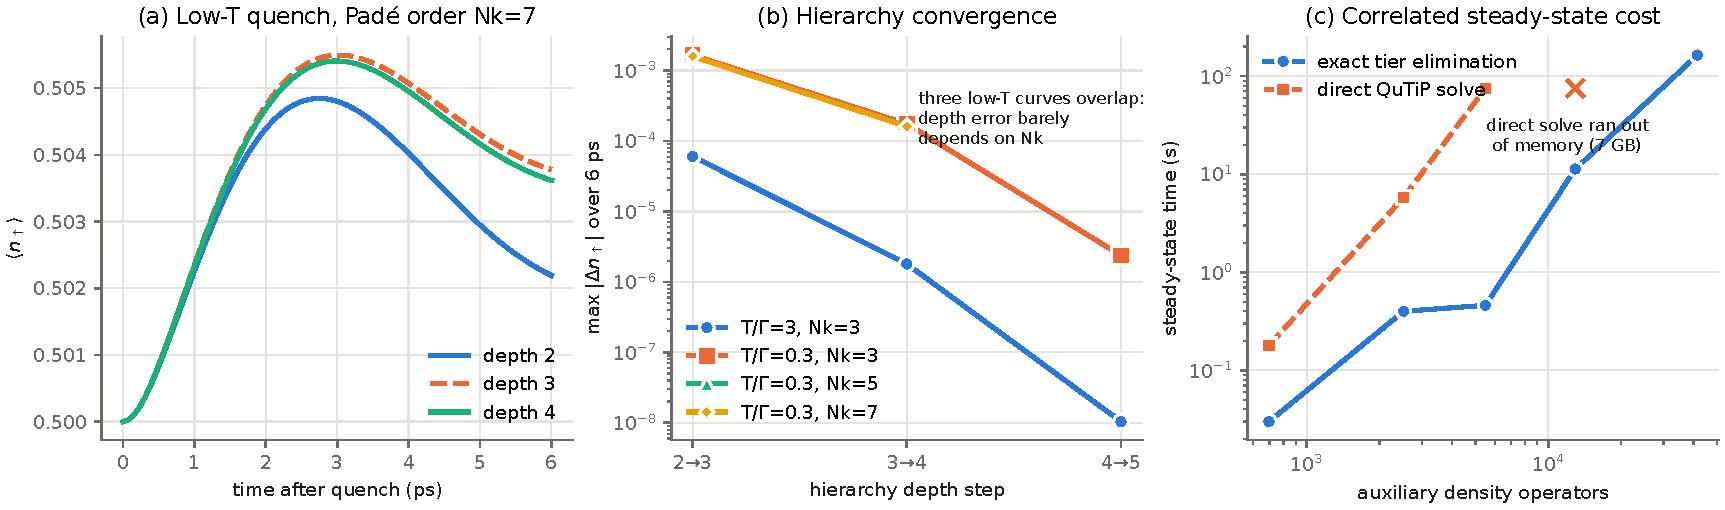
\includegraphics[width=\linewidth]{tier_elimination_convergence.pdf}
\caption{Hierarchy-depth convergence of the quench and cost of preparing the
correlated stationary state, direct versus eliminated.}
\label{fig:conv}
\end{figure}

\subsection{Padé order and integrator}

\begin{table}[h]
\centering\small
\begin{tabular}{lc}
\toprule
check ($T/\Gamma = 0.3$) & $\max_t|\Delta\langle n_\uparrow\rangle|$\\
\midrule
Padé $N_k$ $3\to5$ (depth 4) & $1.57\times10^{-3}$\\
Padé $N_k$ $5\to7$ (depth 4) & $5.10\times10^{-5}$\\
Padé $N_k$ $5\to7$ (depth 3) & $5.07\times10^{-5}$\\
Padé $N_k$ $7\to9$ (depth 3) & $7.44\times10^{-6}$\\
integrator rtol $10^{-10}$ vs $10^{-7}$ ($N_k=7$, depth 3) & $3.5\times10^{-9}$\\
\bottomrule
\end{tabular}
\caption{Padé-order and time-integration checks.}
\label{tab:pade}
\end{table}

Table~\ref{tab:pade} shows that at $T/\Gamma = 0.3$, three Padé poles are not
enough: the $N_k = 3\to5$ change ($1.6\times10^{-3}$) is as large as the depth-2
truncation error, so a low-temperature result with $N_k = 3$ is limited by the bath
expansion, not by the hierarchy depth. The Padé error is also nearly
independent of depth (rows 2--3), so the two error sources can be estimated
separately.

\subsection{Converged reference}

At $T/\Gamma = 0.3$, $N_k = 7$, depth 4, after the $\mu: 0\to0.05$\,meV quench,
\begin{equation}
\langle n_\uparrow\rangle(6\,\mathrm{ps}) = 0.503618,
\end{equation}
with estimated errors of about $2\times10^{-6}$ (depth), $7\times10^{-6}$ (Padé) and
below $10^{-8}$ (integration): a total uncertainty of order $10^{-5}$, about
$160\times$ smaller than the depth-2 truncation error it replaces. All final reduced
density matrices are positive (smallest eigenvalue 0.028) with unit trace.
The full trajectories are stored in the repository and regenerate in about
6 minutes on 2 cores (peak memory 4.5\,GB).

\section{Limitations}

\begin{itemize}
\item The elimination is exact only for the stationary state. After the quench
  the full hierarchy is propagated (29\,s at $N_k = 7$, depth 4).
\item The depth error at $N_k = 7$ is extrapolated from the $N_k = 3$ depth-5 run,
  using the observed $N_k$-independence of the depth error; a direct $N_k = 7$,
  depth-5 calculation was not done.
\item The model has one lead per spin. It is a standard benchmark geometry but not
  the two-lead (source--drain) set-up of transport studies.
\item At points with $\varepsilon-\mu=-U/2$ the occupation stays exactly 0.5 at
  every depth by particle--hole symmetry, so such points are trivial tests and
  should not be used to validate solvers.
\item $D$ is diagonal here because $H_S$ is diagonal in the occupation basis. For a
  general system $D$ is block diagonal with $d^2\times d^2$ blocks, which are
  still cheap to invert but no longer trivially so.
\end{itemize}

\section{Outlook}

The reference gives a fixed target for approximate solvers of non-Markovian
dynamics. The natural next test is whether a neural or reduced-order model,
trained at lower depth, can reproduce $\langle n_\uparrow\rangle(t)$ to the
$10^{-4}$ level at a fraction of the full-hierarchy cost. The same elimination
applies to any HEOM stationary problem, for example steady-state currents in a
two-lead geometry, where the stationary solve is the whole calculation.

\paragraph{Code and data.} Implementation
(\path{src/nonmarkovian_neural_dynamics/tier_elimination.py}), unit tests
against QuTiP, convergence script and figure are in the repository above. The
headline result was reproduced by an independent CI run to 13 digits.

\begin{thebibliography}{9}
\bibitem{TanimuraKubo1989} Y.~Tanimura and R.~Kubo, J.\ Phys.\ Soc.\ Jpn.\ \textbf{58}, 101 (1989).
\bibitem{Tanimura2020} Y.~Tanimura, J.\ Chem.\ Phys.\ \textbf{153}, 020901 (2020).
\bibitem{Jin2008} J.~Jin, X.~Zheng, and Y.~Yan, J.\ Chem.\ Phys.\ \textbf{128}, 234703 (2008).
\bibitem{HuXuYan2010} J.~Hu, R.-X.~Xu, and Y.~Yan, J.\ Chem.\ Phys.\ \textbf{133}, 101106 (2010).
\bibitem{Lambert2023} N.~Lambert \emph{et al.}, Phys.\ Rev.\ Research \textbf{5}, 013181 (2023).
\bibitem{TanimuraWolynes1991} Y.~Tanimura and P.~G.~Wolynes, Phys.\ Rev.\ A \textbf{43}, 4131 (1991).
\bibitem{IshizakiTanimura2005} A.~Ishizaki and Y.~Tanimura, J.\ Phys.\ Soc.\ Jpn.\ \textbf{74}, 3131 (2005).
\end{thebibliography}

\end{document}
